\section{Experiments}

\begin{figure}[t]
%\begin{figure}[t]
  \centering
  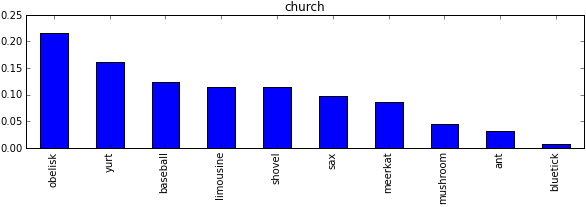
\includegraphics[width=0.5\textwidth]{figs/word2vec_church.png}
  \caption{
    The word2vec similarity scores for \emph{church}. Other structures, such as
    \emph{obelisk} and \emph{yurt} (a type of tent) were the closest in
    similarity. \emph{Bluetick} (a type of dog) was the most distant.
  }
  \label{fig:word2vec_similarities}
\end{figure}

% \begin{table}[!tb]
%   \centering
%   \begin{tabular}{|c|c|c|}
%     \hline
%       & \textbf{1-Hot Labels} & \textbf{Word2Vec Labels} \\
%     \hline
%       \textbf{VGG-16} & 0.2167 & 0.2091 \\
%     \hline
%       \textbf{4-layer CNN} & 0.1091 & 0.1864 \\
%     \hline
%   \end{tabular}
%   \caption{
%     The training results after 50 epochs of using 1-hot labels vs. using soft
%     labels from Word2Vec.
%   }
%   \label{tbl:results}
% \end{table}

% We will evaluate and compare the performance of deep convolutional neural
% networks trained on ImageNet with soft labels and 1-hot labels.
% We will train the VGG-16 model \cite{simonyan2014very} from scratch, and see
% how well it learns using the different labeling schemas. Our goal is to try to
% find the optimal hyperparameters for which soft label training will outperform
% 1-hot labels.
% We will also analyze the errors made by both models to see how semantically
% relevant the models are.
% We plan to use the evaluation method introduced in \cite{zhao2011large} for
% testing semantically relevant errors.

% We will also experiment with pretrained networks and different architectures to
% see how effectively they can learn with soft labels compared to 1-hot labels.
% In \cite{hinton2015distilling} the authors showed that they can use soft labels
% to train simpler models quickly that perform nearly as well as the advanced
% models with many more parameters. We hope to mirror these results, but using
% semantic weights for the learning targets.
% Finally, we plan to experiment with training on fewer examples to see if our
% approach can help in cases where labeled data is limited.

% Throughout all of our experiments, we will compare different schemes for
% obtaining the soft labels. We will use Word2Vec, WordNet, and possibly visual
% similarity, and discover optimal distributions for these weights.
% We hope to look at different linguistic semantic similarity measures and
% compare them with visual similarity measures, and analyze which object
% categories relate well in both the visual and semantic domain.

We consider three class sets, each of which were taken from ImageNet. The first
class set, C5, consists of the following five classes:
\emph{sax},
\emph{church},
\emph{obelisk},
\emph{yurt}, and
\emph{limousine}.
The next class set, C10, consists of the following ten classes:
\emph{sax},
\emph{limousine},
\emph{shovel},
\emph{baseball},
\emph{meerkat},
\emph{church},
\emph{yurt},
\emph{obelisk},
\emph{bluetick}, and
\emph{mushroom}.
The final class set, C10', consists of the following ten classes:
\emph{limousine},
\emph{fiddler crab},
\emph{baseball},
\emph{dalmatian},
\emph{barber chair},
\emph{church},
\emph{lakeside},
\emph{mushroom},
\emph{measuring cup}, and
\emph{projectile}.

The categories for the C5 and C10 class sets were hand-selected to contain
semantically-related labels. Specifically, in C5 \emph{church}, \emph{obelisk},
and \emph{yurt} have stronger semantic relationships to each other than to the
two other classes (see Figure \ref{fig:aff-5_1}).  Similarly, in C10,
\emph{meerkat} and \emph{bluetick} are similar (both are animals).
\emph{Limousine}, \emph{sax}, and \emph{shovel} are all artificially created
instruments for various applications.  Categories \emph{church}, \emph{obelisk},
and \emph{yurt} are also present in this set.  C10' deliberately contains
classes which are less semantically similar to each other.

\begin{figure*}[t]
%\begin{figure}[t]
  \centering
  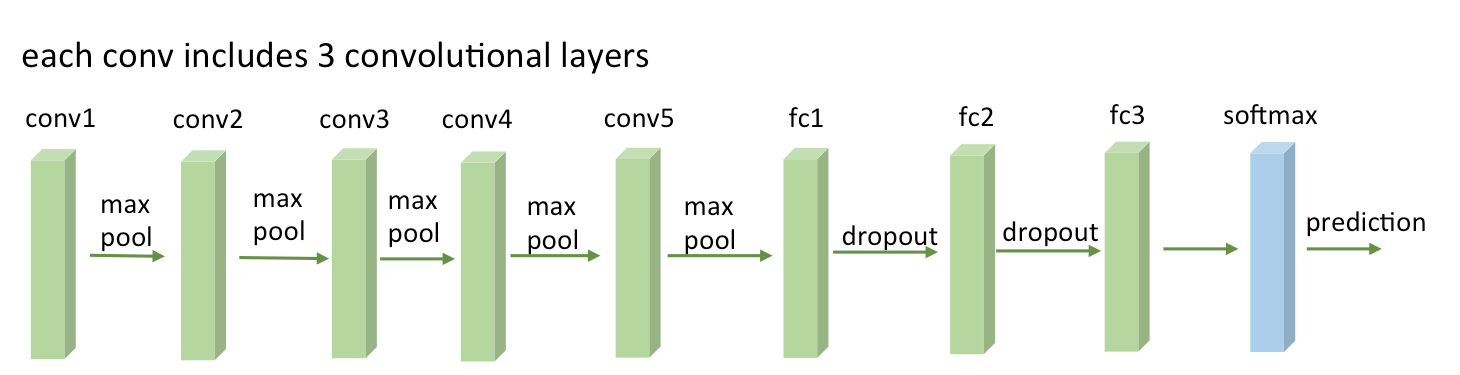
\includegraphics[width=1.0\textwidth]{figs/vgg16arch.png}
  \caption{
      VGGNet architecture. Image credit
      \url{http://blog.christianperone.com/tag/keras/}.
  }
  \label{fig:vgg16arch}
\end{figure*}

For each class set, we train a VGGNet with our proposed soft labeling schemes.
The VGGNet architecture is pictured in Figure \ref{fig:vgg16arch}. The only
modification we made to the architecture was varying the size of the softmax
layer based on the class set size.

Figures \ref{fig:5_1-train_100} and \ref{fig:5_1-train_1260} show results on
C5. We see that soft-labeling schemes consistently outperform the
one-hot labeling scheme and the random labeling scheme for the case of 100
training examples per class. However, the improvement becomes less significant
when the number of training examples per class increases to 1260. This can be
explained by the fact that the additional information encoded in the soft labels
becomes less valuable when the number of training examples increases. This
finding is consistent with \cite{hinton2015distilling}, in which an expert model
(which was trained on one-hot labels) is the proprietor of the soft labels.

\begin{figure}[t]
%\begin{figure}[t]
  \centering
  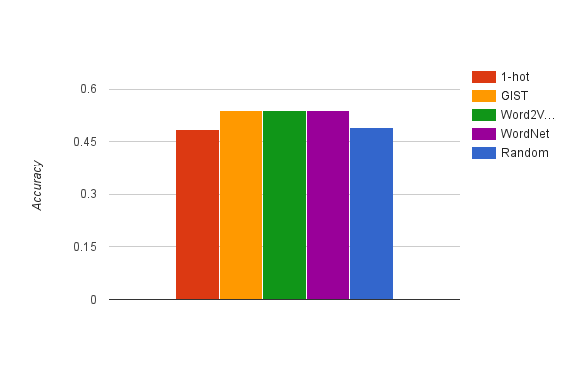
\includegraphics[width=0.5\textwidth]{figs/5_1-train_100.png}
  \caption{
      Performance comparison of all labeling schemes sharing schemes on the C5 class
      set, trained on 100 images per class. Our soft-labeling schemes
      consistently outperform one hot and random labeling schemes, especially
      with a small number of training examples.
  }
  \label{fig:5_1-train_100}
\end{figure}

\begin{figure}[t]
%\begin{figure}[t]
  \centering
  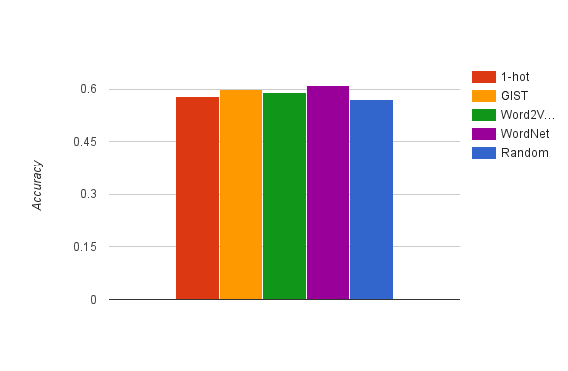
\includegraphics[width=0.5\textwidth]{figs/5_1-train_1260.png}
  \caption{
      Performance comparison of the C5 class set using 1260 training images
      per class.
  }
  \label{fig:5_1-train_1260}
\end{figure}

Figures \ref{fig:10_1-train_100} and \ref{fig:10_1-train_1260} show the
performance of the labeling schemes on C10. Once again we see improved
performance for the soft labeling schemes over one-hot and random. The
performance boost is more significant here than in C5, owing to the fact that
the increase in the number of classes provides soft labels with more
opportunities to convey information in the form of relationships between
classes.

Figure \ref{fig:10_3-train_1260} shows performance on C10'. Because the classes
chosen for this set are not as semantically related, we expected the gains in
performance to be lower. This is true for word2vec, but we still see an
improvement using the WordNet soft labels over 1-hot labels. Further
experimentation needs to be done to analyze why this is the case, but
nevertheless visual and semantic similarities exist among these categories, even
though they not as strong.

\begin{figure}[!tb]
%\begin{figure}[t]
  \centering
  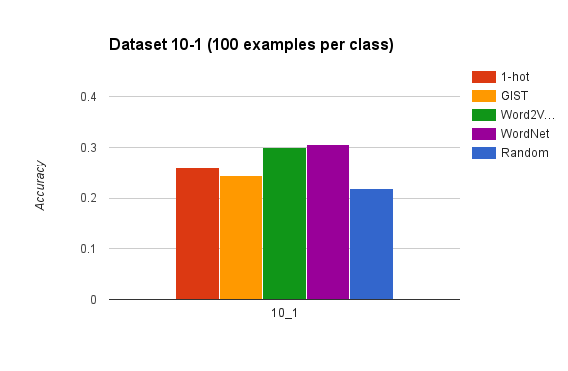
\includegraphics[width=0.5\textwidth]{figs/10_1-train_100.png}
  \caption{
      Performance comparison of the C10 class set using 100 training images
      per class.
  }
  \label{fig:10_1-train_100}
\end{figure}

\begin{figure}[!tb]
%\begin{figure}[t]
  \centering
  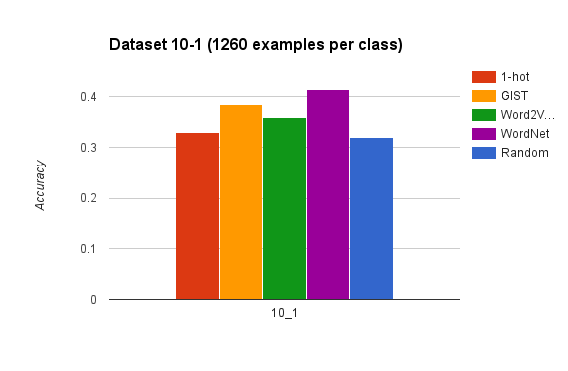
\includegraphics[width=0.5\textwidth]{figs/10_1-train_1260.png}
  \caption{
      Performance comparison of the C10 class set using 1260 training images
      per class.
  }
  \label{fig:10_1-train_1260}
\end{figure}

\begin{figure}[!tb]
%\begin{figure}[t]
  \centering
  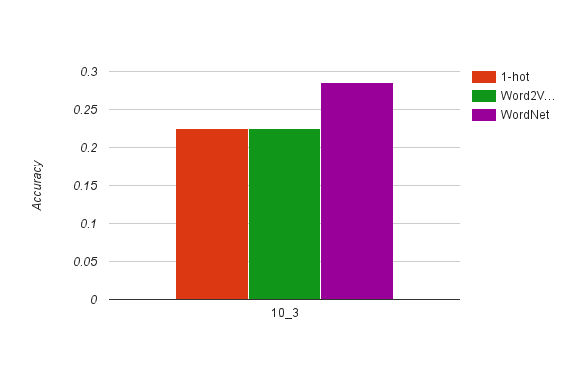
\includegraphics[width=0.5\textwidth]{figs/10_3-train_1260.png}
  \caption{
      Performance comparison of the C10' class set which contains categories
      that are less semantically similar. These are the results after training
      on 1260 images per class.
  }
  \label{fig:10_3-train_1260}
\end{figure}

The fact that GIST soft-labels performed well was a nice surprise for us. Even
though visual similarity between classes is often noisy, it still provides
enough of a signal to improve learning, at least for the 1260 training examples
per-class case.

% As a proof of concept, we trained two models on a small amount of data from
% ImageNet. We used 11 ImageNet classes -
% \emph{
%   saxophone,
%   limousine,
%   shovel,
%   baseball,
%   meerkat,
%   church,
%   yurt,
%   obelisk,
%   bluetick,
%   mushroom,
%   ant
% } -
% each with 100 training examples and 20 test examples.
% Using Word2Vec trained on articles from Google News, we extracted similarity
% scores between these categories. The similarity scores for \emph{church} are
% shown in Figure \ref{fig:word2vec_similarities}.

% We trained the VGG-16 model as well as a simpler four-layer CNN on this data
% set. Our average results over three experimental trials can be seen in Table
% \ref{tbl:results}.
% While the results for the VGG-16 model are similar in both cases, there is a
% clear boost in performance on the simpler model. Our naivly-selected soft
% labels perform almost as well as VGG-16 despite being a significantly inferior
% architecture.
% The overall poor performance can be attributed to the tiny training data set.

% Naturally, we will run experiments with much larger training sets and we will
% search for the best hyperparameters.
% We will also work on improving the design of the soft labels, which were not
% adjusted at all for this experiment - we just took the cosine similarity
% between the raw Word2Vec features.


\begin{figure}[t]
%\begin{figure}[t]
  \centering
  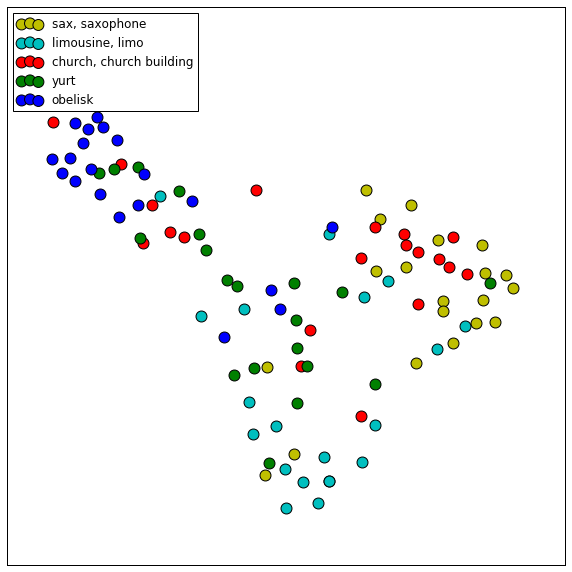
\includegraphics[width=0.5\textwidth]{figs/tsne.png}
  \caption{
      t-SNE visualization of predicted softmax probabilities for C5 test set.
      Notice \emph{yurt} and \emph{obelisk,} two labels with a high semantic
      score, cluster together.
  }
  \label{fig:tsne}
\end{figure}

\begin{table}[!tb]
    \centering
    \begin{tabular}{lrr}
         & WN-PATH & WN-ZHAO\\
        \hline
        WordNet + GIST & 0.261114 & 0.456478\\
        word2vec & 0.2995 & 0.550523\\
        WordNet & 0.36027 & \textbf{0.581415}\\
        Dependency & 0.091352 & 0.394429\\
        1-Hot & \textbf{0.361664} & 0.533101\\
    \end{tabular}
  \caption{
      Semantic evaluation on misclassified examples. Models trained with soft
      labels generally make more semantically meaningful errors.
  }
  \label{tbl:semantic_misses}
\end{table}

Table \ref{tbl:semantic_misses} illustrates the quality of mistakes each model
makes. The \emph{Dependency} soft labels were derived in an identical way to the
\emph{word2vec} model, but we used word vectors from \cite{levy2014dependency}.
For the WordNet+GIST soft labels, we averaged WordNet and GIST affinity
matrices. WN-ZHAO and WN-PATH are affinity matrices computed with equations
\ref{eq:wordnet_dist} and \ref{eq:path_dist}, respectively. To compute scores,
we use a similar semantic evaluation metric to \cite{zhao2011large}, but with
the following deviation: for an affinity matrix $A$, a prediction for class $i$
when the correct class is $j$ nets a score of $A_{ij}$ for that image. For
example, if $i = j$, this corresponds to a correct prediction and the model is
awarded 1 point (because $A_{ii}$ = 1 for all $i$), which is identical to
standard accuracy. However, if the model makes an incorrect prediction (i.e. $i
\neq j$), then the model is awarded a score of $A_{ij}$.  Recall that $A_{ij}$
is the affinity for classes $i$ and $j$ and will be large when the two classes
are similar. Hence the model gets more credit for predicting related classes and
less credit when predicting an unrelated class.

We can see that the model trained on one hot labels performs highest on WN-PATH,
but both word2vec and WordNet perform higher on WN-ZHAO. We believe performance
is higher for WordNet and word2vec on WN-ZHAO because of the relative uniformity
(diffuse) of the WN-PATH affinity matrix. Because WN-PATH is more diffuse, the
one-hot model does is not penalized as harshly for making bad semantic mistakes,
whereas it is penalized much more harshly with WN-ZHAO because WN-ZHAO is more
sparse. We acknowledge that WordNet model's score on WN-ZHAO is likely inflated
because it was was trained directly on the WN-ZHAO affinity matrix, but we are
pleased to see that word2vec also outperforms one-hot and requires no such
disclaimer.

It can be seen that WordNet+GIST and Dependency do quite poorly. For
WordNet+GIST, we expected averaging WordNet and GIST affinity matrices to reduce
the performance loss in cases of disagreement between semantic and visual
similarity. However, we need to experiment further with taking different linear
combinations of the two metrics. As for Dependency, qualitatively we noticed
poor rankings for class similarity (e.g. every class had \emph{yurt} as being
most similar), which we believe to be responsible for it reprehensible
performance.

Figure \ref{fig:tsne} shows a t-SNE plot of the predicted softmax probability
vectors for the C5 class set with word2vec soft labels. We notice that images of
\emph{yurts} and \emph{obelisks} are clustered close together, indicating that
these two labels received high probability mass \emph{jointly}. As an aside, we
would like to point out that t-SNE plots are typically performed on the final
hidden layer of a CNN, but performing a t-SNE plot on the softmax probabilities
more accurately reflects the goals of this work.

% \begin{table*}[t]
%     \centering
%     \begin{tabular}{lrrrrr}
%          & WN-PATH & WN-WUP & WN-ZHAO & GIST & 1-HOT\\
%         \hline
%         WordNet + GIST & 0.603798 & 0.729889 & 0.716476 & 0.703609 & 0.57\\
%         WordNet & 0.585442 & 0.725779 & 0.710825 & 0.678581 & 0.55\\
%         word2vec & 0.624362 & 0.755722 & 0.742397 & 0.708035 & 0.59\\
%         Dependency Embeddings & 0.535218 & 0.71633 & 0.696365 & 0.652365 &
%         0.49\\
%         One Hot & 0.622404 & 0.74834 & 0.735746 & 0.711471 & 0.59\\
%     \end{tabular}
%     \caption{
%         Semantic evaluation numbers for different soft labeling schemes. The
%         word2vec labeling scheme achieves the same raw accuracy as one hot, but
%         scores higher on WordNet metrics.
%     }
%   \label{tbl:semantic_eval}
% \end{table*}


%\subsection{CNN Architecture}
%
%TODO.
